
\documentclass[12pt]{article}
\usepackage{geometry}
 \geometry{letterpaper,left=25mm,top=25mm,right=25mm}
\usepackage[utf8]{inputenc}
\usepackage[spanish]{babel} %Poner algunas palabras reservadas en español
\usepackage{authblk} %Poner instituto en la portada
%Paquetes para símbolos matematicos
\usepackage{amsmath}
\usepackage{mathtools}
\usepackage{amsthm}
\usepackage{amssymb}
\usepackage{bbm}
\usepackage[]{algorithm2e} %Paquete para algoritmos
\usepackage{enumerate}
%Paquete para imagenes
\usepackage{graphicx}
\graphicspath{{img/}}
%Paquete para teoremas
\newtheorem*{thm}{Teorema}
%Quitar la sangria
\setlength{\parindent}{0cm}

\title{Tarea 2}
\author{Fernando Márquez Pérez \\ Juan Antonio Jasso Oviedo \\ Emiliano Dom\'inguez Cruz}
\date{04/10/2019}
\affil{Facultad de Ciencias\\UNAM}

\begin{document}
\begin{titlepage}
    \maketitle
\end{titlepage}

%EJERCICIO 1 ----------------------------------------------------------------------------------
1. Determine si las siguientes funciones son continuas en \(x_0\).

\begin{enumerate}[\hspace{9px} a)]
    \item
    \( f(x)=
    \begin{cases}
        \sqrt{x^2-1}\text{, si} \ x \geq 1\\
        x^2-2x+1\text{, si} \ x \in [0,1]
    \end{cases}
    \)
    en $x_0 = 1$\\
    \item
    \( h(x)=
    \begin{cases}
        \frac{|x|}{x}\text{, si} \ x \neq 0\\
        1\text{, si} \ x=0\\
    \end{cases}
    \)
    en $x_0=0$
    \item
    \( g(x)=
    \begin{cases}
        \sqrt{1-x^2}\text{, si} \ x \in [0,1]\\
        -\sqrt{1-(x-2)^2}\text{, si} \ x \in [1,2]
    \end{cases}
    \)
    en $x_0=1$
\end{enumerate}

%EJERCICIO 2 ----------------------------------------------------------------------------------
2. Se inyecta un fármaco a un paciente cada 12 horas. En la Fig. 1 se muestra la concentración $c(t)$ del fármaco en el torrente sanguieo después de $t$ horas.
\begin{figure}[h]
    \centering
    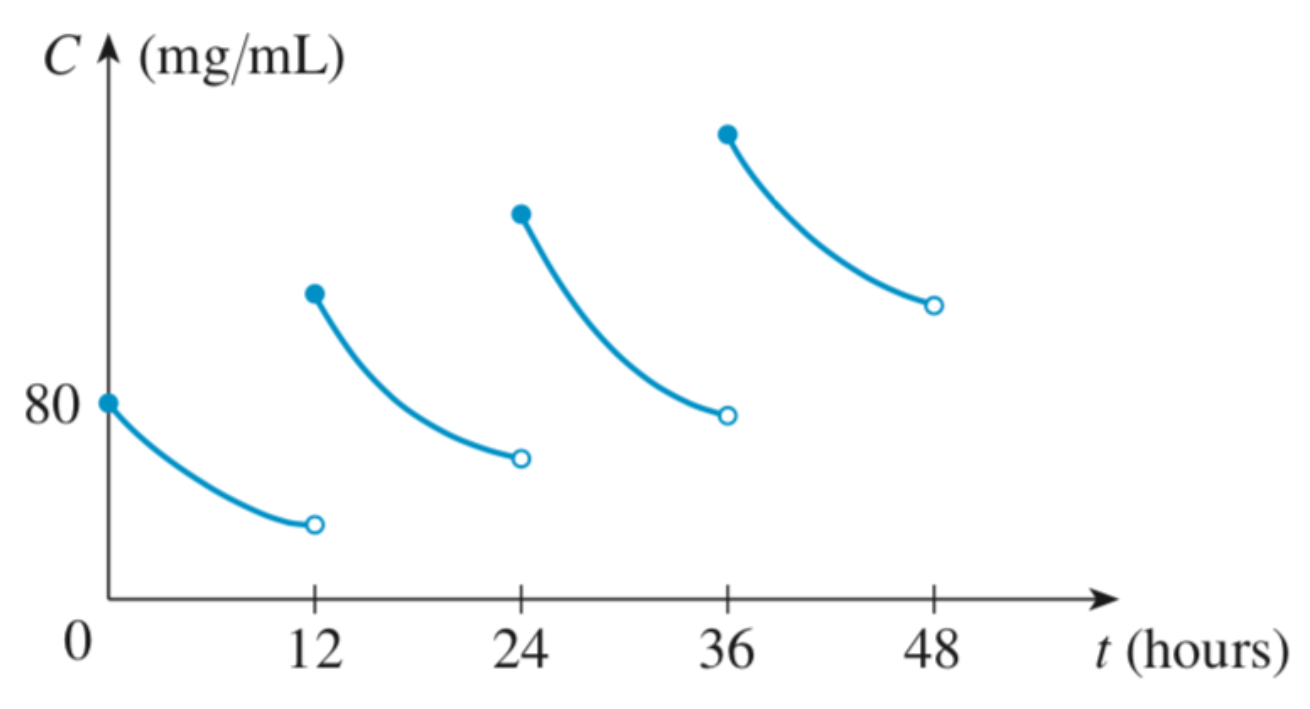
\includegraphics[width=0.5\textwidth]{fig1}
    \caption{Concentraci\'on de f\'armaco}
    %Para referenciarla usar \ref{fig1}
    \label{fig1}
\end{figure}
\begin{enumerate}[\hspace{9px} a)]
    \item ¿Para qué valores de $t$, $c(t)$ tiene discontinuidades?
    \item ¿Qué tipo de discontinuidades tiene?
\end{enumerate}

%EJERCICIO 3 ----------------------------------------------------------------------------------
3. Mostrar que existe algún número $x$, tal que:

\begin{enumerate}[\hspace{9px} a)]
    \item \(\sin x = x-1\)
    \item \(x^{179}+\displaystyle\frac{163}{1+x^2+\sin^2 x}=119\)
    \item \(\cos x - \displaystyle\frac{1}{2}=x-1\)
    \item \((2x^2-2)^2=-x+1\)
\end{enumerate}

%EJERCICIO 4 ----------------------------------------------------------------------------------
4. Vea si en los siguientes incisos se cumple el teorema de valor intermedio y, en ese caso, calcula un valor intermedio.

\begin{enumerate}[\hspace{9px} a)]
    %EJERCICIO A
    \item \(f(x)=x^3\) en $[-1,1]$\\

        Obtenemos $f(-1)$ y $f(1)$:
        \begin{align*}
            &f(-1) = (-1)^3 = -1  &&f(1) = (1)^3 = 1
        \end{align*}

        Sabemos que $f$ es un polinomio de grado 3 y que todos los polinomios son continuos en $\mathbbm{R}$, por ende, $f$ es continua en $[-1,1]$.\\

        Como $f(-1) < 0 < f(1)$ y $f(x)$ es continua en $[-1,1]$. Podemos usar el \textbf{Teorema del Valor Intermedio} para decir que: \(\exists \ x_0 \in (-1,1) : \ f(x_0)=0\).\\

        Ahora buscamos a $x_0$:
        \begin{equation*}
            f(x_0)=0 \Rightarrow (x_0)^3 = 0 \Rightarrow (x_0)(x_0)(x_0)=0 \Rightarrow x_0=0
        \end{equation*}

        \textbf{$\mathbf{\therefore \ f(x)}$ cumple el Teorema del Valor Intermedio en el intervalo dado. Un valor intermedio es $\mathbf{x_0=0}$.}\\

    %EJERCICIO B
    \item \(g(x)=x^3\) en $[0,2]$\\

        Obtenemos $g(0)$ y $g(2)$:
        \begin{align*}
            &g(0)=(0)^3=0 &&g(2)=(2)^3=8
        \end{align*}

        Estrictamente hablando, $g(x)$ no cumple el \textbf{Teorema del Valor Intermedio} porque \(g(0) < 0 < g(2)\) no es verdad porque $g(0)=0$. Pero es eso se debe a que justo el intervalo toma al $x_0$ que cumple $g(x_0)=0$: $\mathbf{x_0=0}$\\

    %EJERCICIO C
    \item \(h(x)=x^2+4x+4\) en $[0,1]$\\

        Obtenemos $h(0)$ y $h(1)$:
        \begin{align*}
            &h(0)=(0)^2+4(0)+4=4 &&h(1)=(1)^2+4(1)+4=1+4+4=9
        \end{align*}

        Como $h$ es un polinomio, es continua en $[0,1]$.\\

        Tenemos, entonces, que \(h(0) > 0 < h(1)\). Como esto no cumple el \textbf{TVI}, buscamos valores dentro de $[0,1]$ que puedan cumplirlo.\\

        Proponemos el intervalo $\left[\frac{1}{2},1\right] \in [0,1]$\\

        Obtenemos \(h\left(\displaystyle\frac{1}{2}\right)\): \quad \(\left(\displaystyle\frac{1}{2}\right)^2+4\left(\displaystyle\frac{1}{2}\right)+4 = \left(\displaystyle\frac{1}{4}\right)+2+4 = \displaystyle\frac{1}{4}+\displaystyle\frac{24}{4}=\displaystyle\frac{25}{4}\)
        \\

        Como \(h\left(\displaystyle\frac{1}{2}\right) > 0 < h(1)\) podemos concluir que:\\

        \textbf{$h(x)$ NO cumple el Teorema del Valor Intermedio en el intervalo dado.}\\

        Lo que tiene sentido porque si buscamos las raices de $f(x)$ obtendremos:

        \begin{equation*}
            h(x_0) \Rightarrow x_0^2+4x_0+4=0 \Rightarrow (x_0+2)^2=0 \Rightarrow x_0+2=0 \Rightarrow x_0=-2
        \end{equation*}\\

    %EJERCICIO D
    \item \(k(x)=3x^2-x-1\) en $[-1,1]$\\

        Obtenemos $k(-1)$ y $k(1)$:
        \begin{align*}
            &k(-1)=3(-1)^2-(-1)-1=3(1)+1-1=3 \\
            &k(1)=3(1)^2-1-1=3(1)-1-1=3-2=1
        \end{align*}

        Como $k$ es un polinomio, es continua en $[-1,1]$.\\

        Tenemos, entonces, que \(k(-1) > 0 < k(1)\). Como esto no cumple el \textbf{TVI}, buscamos valores dentro de $[0,1]$ que puedan cumplirlo.\\

        Proponemos el intervalo $[0,1] \in [-1,1]$\\

        Obtenemos $k(0)$: \quad \(3(0)^2-0-1=0-0-1=-1\)\\

        Como tenemos que \(k(0) < 0 < k(1)\) y que $k$ es continua en el intervalo. Podemos usar el \textbf{Teorema del Valor Intermedio} para decir que: \(\exists \ x_0 \in (-1,1) : \ k(x_0)=0\).\\

        Ahora buscamos $x_0$: \quad $3x^2-x-1=0$\\

        Para encontrar $x_0$ cerramos el intervalo:
        \[k\left(\displaystyle\frac{1}{2}\right) = 3\left(\frac{1}{2}\right)^2-\left(\frac{1}{2}\right)-1=\frac{3}{4}-\frac{6}{4}=-\frac{3}{4}\]

        Si proponemos el intervalo $\left[\displaystyle\frac{1}{2},1\right]$ Tenemos que:

        \(k\left(\displaystyle\frac{1}{2}\right) < 0 < k(1) \Longrightarrow -\displaystyle\frac{3}{4} <0<1\).\\

        Como seguimos cumpliendo el TVI. Seguimos cerrando en intervalo:

        \[k\left(\displaystyle\frac{3}{4}\right)=3\left(\frac{3}{4}\right)^2-\left(\frac{3}{4}\right)-1=\frac{27}{16}-\frac{7}{4}=\frac{27}{16}-\frac{28}{16}=-\frac{1}{16}\]

        $-\displaystyle\frac{1}{16}$ es un valor muy cercano a 0. Por lo que podemos decir que $x_0 \approx \displaystyle\frac{3}{4}$

        Lo que tiene sentido porque si obtenemos las raices de $k$ usando la f\'ormula general, tenemos que:

        \(x=\displaystyle\frac{-b\pm \sqrt{b^2-4ac}}{2a}\) \quad Donde $a=3$, $b=-1$ y $c=-1$.

        \begin{align*}
            x&=\frac{-(-1)\pm \sqrt{(-1)^2-4(3)(-1)}}{2(3)}\\
            &=\frac{1\pm \sqrt{1+12}}{6}\\
            &=\frac{1\pm \sqrt{13}}{6}
        \end{align*}
        y \ \(\displaystyle\frac{1+\sqrt{13}}{6} \approx \frac{3}{4}\)\\

        \textbf{$\mathbf{\therefore \ k(x)}$ cumple el Teorema del Valor Intermedio en el intervalo dado. Un valor intermedio es $\mathbf{x_0=\displaystyle\frac{1+\sqrt{13}}{6}}$.}\\

\end{enumerate}

%EJERCICIO 5 ----------------------------------------------------------------------------------
5. Pruebe que las ecuaciones dadas, tienen una raíz en el intervalo que se señala.

\begin{enumerate}[\hspace{9px} a)]
    \item \(x^3+7x^2-3x-5=0\) en $[-3.2,0.1]$
    \item \(x^5-4x^3+x^2-1=0\) en $[-2.1,1.5]$
    \item \(x\sin x-\displaystyle\frac{1}{2}=0\) en $[-1,2]$
    \item \(x\cos x+\displaystyle\frac{1}{2}=0\) en $[-1,3.5]$
\end{enumerate}

%EJERCICIO 6 ----------------------------------------------------------------------------------
6. Partiendo de la definición de derivada, mostrar que:

\begin{enumerate}[\hspace{9px} a)]
    \item si \(f(x)=\displaystyle\frac{1}{x}\), entonces \(f'(a)=-\displaystyle\frac{1}{a^2}\) para \(a \neq 0\)
    \item si \(f(x)=\displaystyle\frac{1}{x^2}\), entonces \(f'(a)=-\displaystyle\frac{2}{a^3}\) para \(a \neq 0\)
    \item si \(f(x)=\sqrt{x}\), entonces \(f'(a)=-\displaystyle\frac{1}{2\sqrt{a}}\) para \(a > 0\)
\end{enumerate}

%EJERCICIO 7 ----------------------------------------------------------------------------------
7. Encontrar la ecuación de la recta tangente en el punto \((a,f(a))\) para las siguiente funciones.

\begin{enumerate}[\hspace{9px} a)]
    \item \(f(x)=\displaystyle\frac{1}{x}\) para \(a \neq 0\)
    \item \(f(x)=\displaystyle\frac{1}{x^2}\) para \(a \neq 0\)
    \item \(f(x)=\sqrt{x}\) para \(a > 0\)
\end{enumerate}

%EJERCICIO 8 ----------------------------------------------------------------------------------
8. Calcular \(f'(x)\) para cada una de las siguientes funciones (sin importar los dominios de \(f\) y \(f'\)).

\begin{enumerate}[\hspace{9px} a)]
    \item \(f(x) = \sin(x+x^2)\)
    \item \(f(x) = \sin(x) + \sin(x^2)\)
    \item \(f(x) = \sin(\cos(x))\)
    \item \(f(x) = \sin(\sin(x))\)
    \item \(f(x) = \sin(x+\sin(x))\)
    \item \(f(x) = \sin(\cos(\sin(x)))\)
    \item \(f(x) = \sin\left(\displaystyle\frac{\cos(x)}{x}\right)\)
    \item \(f(x) = \displaystyle\frac{\sin(\cos(x))}{x}\)
    \item \(f(x) = \displaystyle\frac{\cos(\cos(x))}{x}\)
\end{enumerate}

%EJERCICIO 9 ----------------------------------------------------------------------------------
9. Dadas las siguiente funciones, encontrar un punto que satisfada el teorema de Rolle.

\begin{enumerate}[\hspace{9px} a)]
    \item \(f: [-2,0] \rightarrow \mathbbm{R} \ \text{tal que} \ f(x)=x^2+2x+1\)
    \item \(f: [0,2] \rightarrow \mathbbm{R} \ \text{tal que} \ f(x)=x^2-2x+1\)
    \item \(f: [-2,0] \rightarrow \mathbbm{R} \ \text{tal que} \ f(x)=\displaystyle\frac{1}{x^2+2x+1}\)
    \item \(f: [0,2] \rightarrow \mathbbm{R} \ \text{tal que} \ f(x)=\displaystyle\frac{1}{x^2-2x+1}\)
\end{enumerate}

%EJERCICIO 10 ----------------------------------------------------------------------------------
10. Dada las siguien funciones, encontrar un punto que satisfaga el teorema del Valor Medio.

\begin{enumerate}[\hspace{9px} a)]
    \item \(f: [-1,1] \rightarrow \mathbbm{R} \ \text{tal que} \ f(x)=x^{4/3}\)
    \item \(f: [-1,2] \rightarrow \mathbbm{R} \ \text{tal que} \ f(x)=x^2-1\)
    \item \(f: [0,2] \rightarrow \mathbbm{R} \ \text{tal que} \ f(x)=x^3-2x-1\)
    \item \(f: [-2,0] \rightarrow \mathbbm{R} \ \text{tal que} \ f(x)=x^3-2x+2\)
\end{enumerate}

%EJERCICIO 11 ----------------------------------------------------------------------------------
11. Calcular los siguientes l\'imites. Analice si se puede aplicar la regla de L'H\^opital.

\begin{enumerate}[\hspace{9px} a)]
    \item \(\displaystyle\lim_{x \to 0}\frac{x}{\tan(x)}\)
    \item \(\displaystyle\lim_{x \to 0}\frac{\cos^2(x)-1}{x^2}\)
    \item \(\displaystyle\lim_{x \to 0}\frac{b^2\cos(ax)}{x}\)
    \item \(\displaystyle\lim_{x \to 0}\frac{\sqrt{x+1}-1}{x}\)
    \item \(\displaystyle\lim_{x \to 1}\frac{2x^2-4x+2}{5x^2-10x+5}\)
    \item \(\displaystyle\lim_{x \to 0}\frac{x-\sin(x)}{x^2}\)
\end{enumerate}

%EJERCICIO 12 ----------------------------------------------------------------------------------
12. Para cada una de las siguientes funciones, hallar $f'(f(x))$.

\begin{enumerate}[\hspace{9px} a)]
    \item \(f(x)=\displaystyle\frac{1}{1+x}\)
    \item \(f(x)=\sin(x)\)
    \item \(f(x)=x^2\)
    \item \(f(x)=17\)
\end{enumerate}

%EJERCICIO 13 ----------------------------------------------------------------------------------
13. Para cada una de las siguientes funciones, hallar $f(f'(x))$.

\begin{enumerate}[\hspace{9px} a)]
    \item \(f(x)=\displaystyle\frac{1}{x}\)
    \item \(f(x)=x^2\)
    \item \(f(x)=17x\)
    \item \(f(x)=17\)
\end{enumerate}

%EJERCICIO 14 ----------------------------------------------------------------------------------
14. Para cada una de las siguiente funciones, hallar el m\'aximo y el m\'inimo en los intervalos indicados, hallando los puntos del intervalo en que la derivada es cero y comparando los valores en estos puntos con los valores en los extremos.

\begin{enumerate}[\hspace{9px} a)]
    \item \(f(x)=x^3-x^2-8x+1\) sobre $[-2,2]$
    \item \(f(x)=\displaystyle\frac{x+1}{x^2+1}\) sobre $\left[-1,\frac{1}{2}\right]$
    \item \(f(x)=x^3+x+1\) sobre $[-1,1]$
    \item \(f(x)=\displaystyle\frac{x}{x^2-1}\) sobre $[0,5]$
\end{enumerate}

%EJERCICIO 15 ----------------------------------------------------------------------------------
15. Cada una de las figuras siguientes, representan la gr\'afica de la derivada de una funci\'on $f$. Hallar todos los m\'aximos y m\'inimos locales de la funci\'on $f$ correpondiente, adem\'as diga cuando $f$ es creciente o decreciente.

\begin{enumerate}[\hspace{9px} a)]
    \item Gr\'afica de la derivada de $f$.\\
        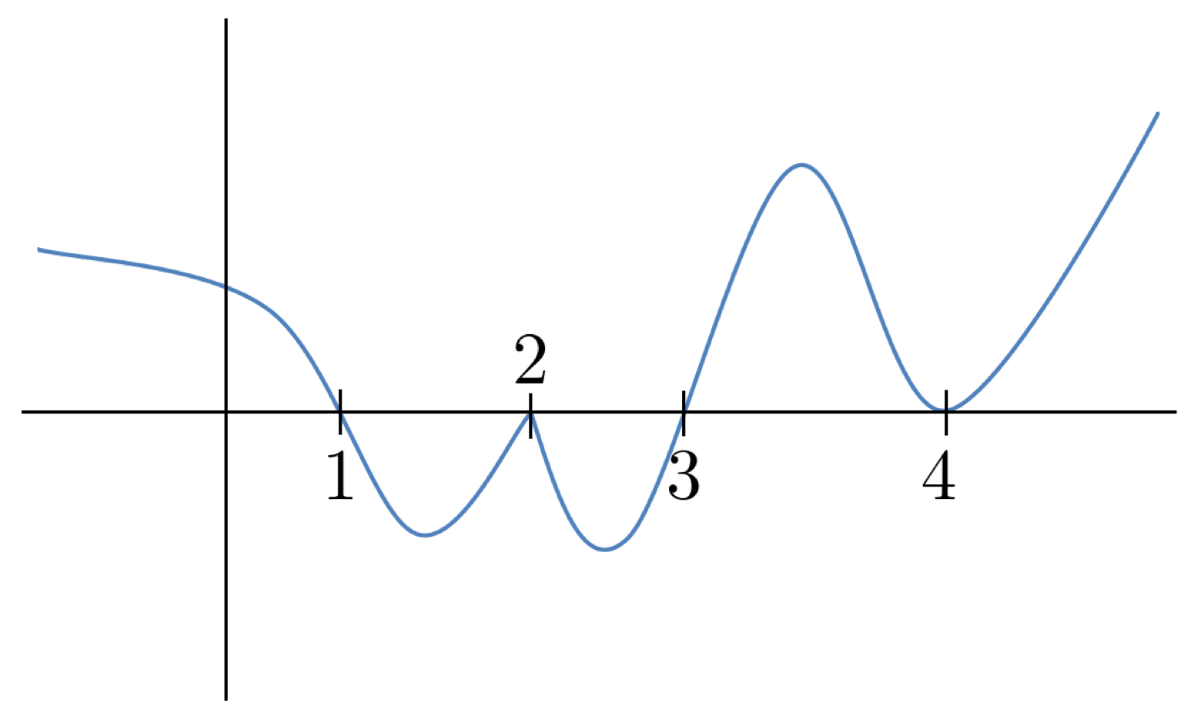
\includegraphics[width=0.5\textwidth]{ejer-a}
    \item Gr\'afica de la derivada de $f$.\\
        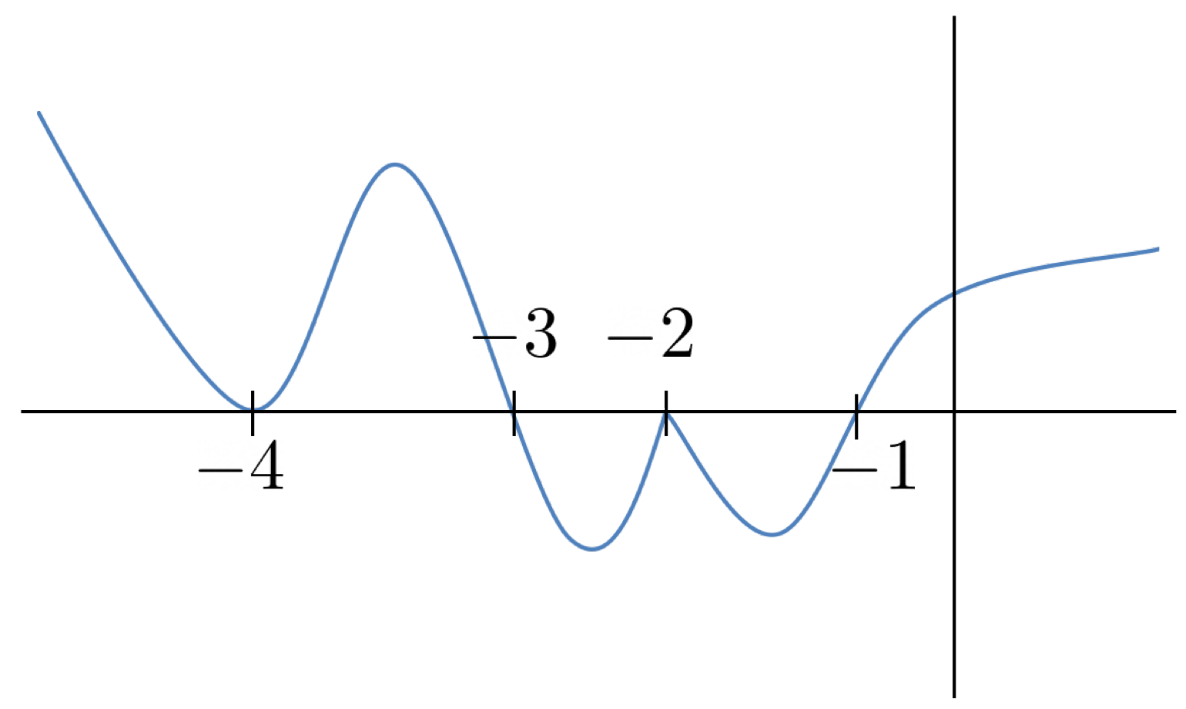
\includegraphics[width=0.5\textwidth]{ejer-b}
    \item Gr\'afica de la derivada de $f$.\\
        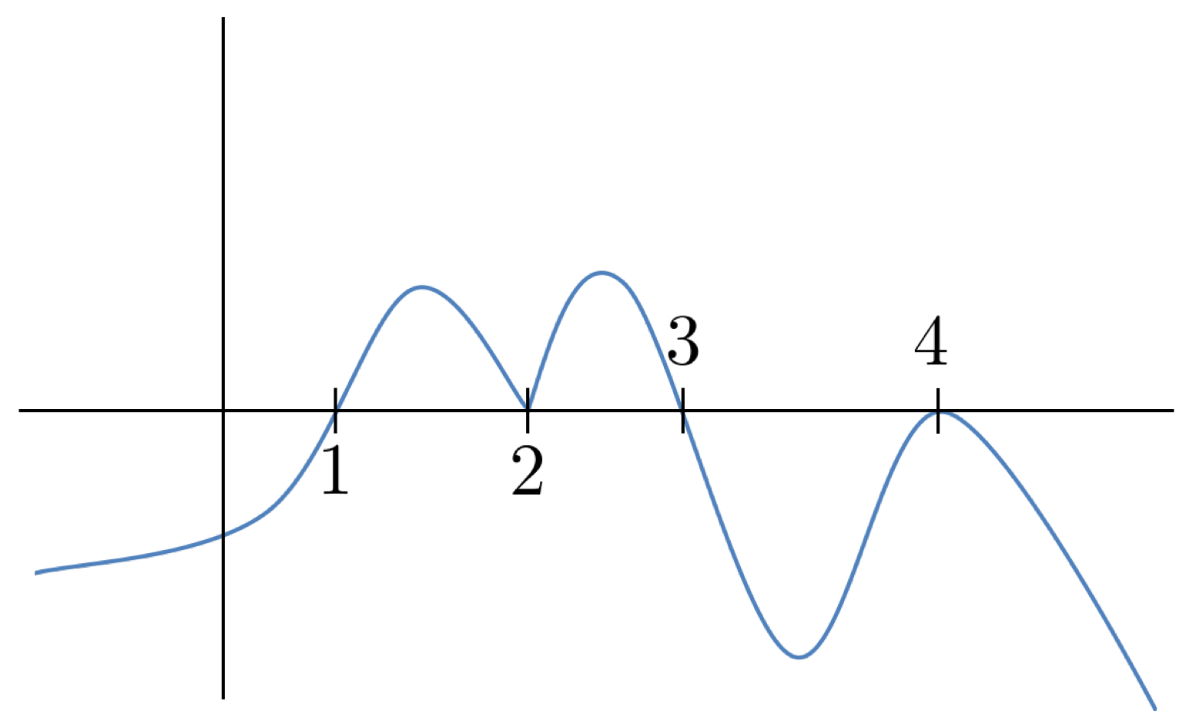
\includegraphics[width=0.5\textwidth]{ejer-c}
    \item Gr\'afica de la derivada de $f$.\\
        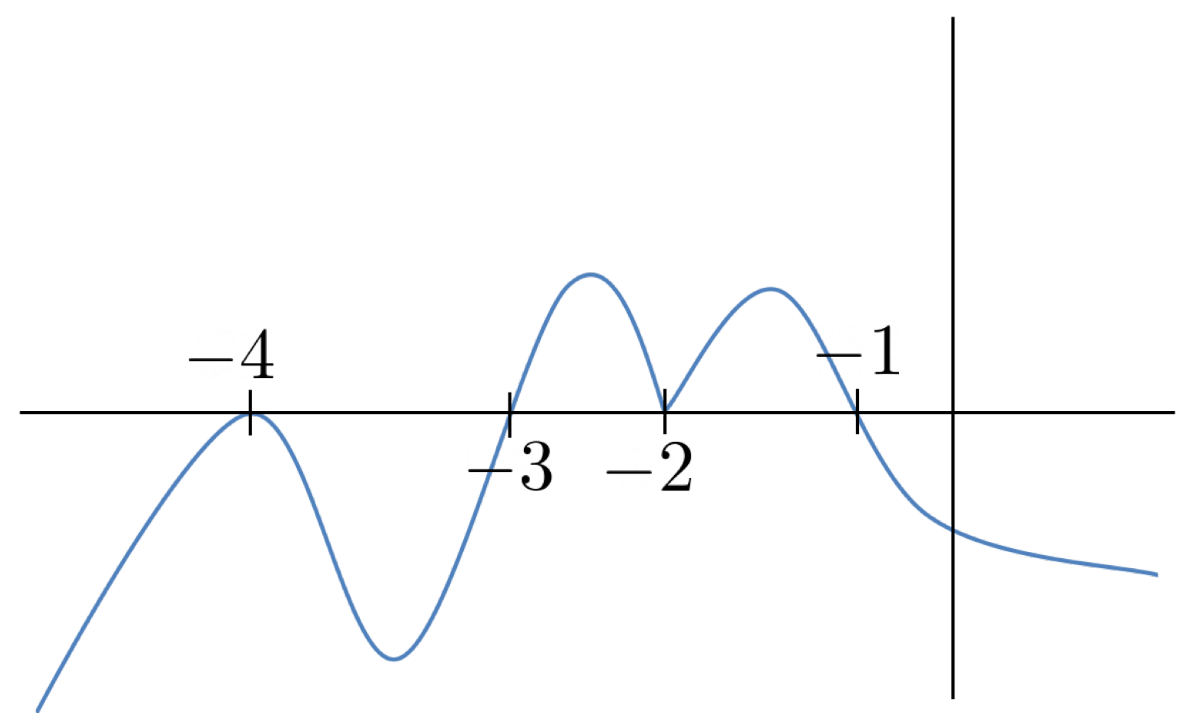
\includegraphics[width=0.5\textwidth]{ejer-d}
\end{enumerate}

%EJERCICIO 16 ----------------------------------------------------------------------------------
16. Utiliza los resultados sobre el significado de la derivada para esbozar la gr\'afica de las siguientes funciones (aplicar criterios de la primera y la segunda derivada).

\begin{enumerate}[\hspace{9px} a)]
    \item \(f(x)=x+\displaystyle\frac{1}{x}\)
    \item \(f(x)=x+\displaystyle\frac{3}{x^2}\)
    \item \(f(x)=\displaystyle\frac{x^2}{x^2-1}\)
    \item \(f(x)=\displaystyle\frac{1}{x^2+1}\)
\end{enumerate}

%EJERCICIO 17 ----------------------------------------------------------------------------------
17. Mostrar que:

\begin{enumerate}[\hspace{9px} a)]
    \item La suma de un n\'umero real positvio y su rec\'iproco es por lo menos 2.
    \item Entre todos los rect\'angulos de igual per\'imetro, el de mayor \'area es el cuadrado.
    \item Entre todos los rect\'angulos con la misma \'area, el cuadrado es el de per\'imetro m\'inimo.
    \item Entre todos los rect\'angulos que pueden inscribirse en una circunferencia, el cuadrado es el de \'area m\'axima.
    \item La raz\'on de variac\'on del volumen de una esfera rexpecto a su radio, es igual a su \'area.
\end{enumerate}

%EJERCICIO 18 ----------------------------------------------------------------------------------
18. Encuentre el punto para el cual:

\begin{enumerate}[\hspace{9px} a)]
    \item La recta tangente a la par\'abola \(f(x)=x^2-7x+3\), es paralela a la recta \(5x+3y-3=0\)
    \item La recta tangente a la par\'abola \(f(x)=x^2-7x+3\), es paralela a la recta \(3x-y-4=0\)
    \item La recta tangente a la pa\'rabola \(f(x)=x^2-7x+3\), es paralela a la recta \(2x+3y-3=0\)
\end{enumerate}

\vfill

%EJERCIO 8
8.Calcular $f'(x)$ para cada una de las siguientes funciones (sin importar los dominios de $f(x)$ y de $f'(x)$).
%EJERCIO A
%    \begin{align*}
        Recordamos por la regla de la cadena primero derivamos sin() y posterormente lo multiplicamos por la derivada de cos(x)\\
        Tenemos\\
        g(x)=sin(cos(x))\\
        g'(x)=cos(cos(x)) \ \ \  %&&\text{Por el teorema que probamos en clase de f(x)=sin(x) entonces f'(x)=cos(x)}\\
        Observamos\\
        h(x)=cos(x)  \ \ \ %&&\text{Por el teorema que probramos en clase de f(x)=cos(x) entonces f'(x)=-sin(x}\\
        h'(x)=-sin(x)\\
        es decir\\
        f'(x)=(cos(cos(x)))(-sin(x)) \ \ \ %&&\text{Por la regla de la cadena se multiplican}\\

%    \end{align*}


%EJERCIO F
%    \begin{align*}
        Recordamos por la regla de la cadena primero derivamos sin(cos(sin(x))) y posteriormente multiplicamos por la derivada de cos(sin(x)) y posteriormente por sin(x) \\
        Tenemos,\\
        g(x)=sin(cos(sin(x)))\\
        g'(x)=cos(cos(sin(x))) \ \ \ %&&\text{Por el teorema que probamos en clase}\\
        Además, tambíen tenemos,\\
        h(x)=cos(sin(x))\\
        h'(x)=-sin(sin(x)) \ \ \ %&&\text{Por el teorema que probamos en clase}\\
        Posteriormente\\
        t(x)=sin(x)\\
        t'(x)=cos(x) \ \ \ %&&\text{Por el teorema que probamos en clase}\\
        es decir\\
        f'(x)=cos(cos(sin(x)))*-sin(sin(x))*cos(x) \ \ \ %&&\text{Por la regla de la cadena se multiplican}\\
%    \end{align*}

%EJERCIO I

%    \begin{align*}
        Observamos\\
        f(x)=g(x)/h(x)  \ \ \ %&&\text{con g(x)=cos(cos(x)) y h(x)=x}\\
        Recordamos\\
        $f'(x)=((h(x)*g'(x))-(g(x)*h'(x)))/g(x)^2$ \ \ \ %&&\text{por el teorema que probamos en clase}\\
        Observamos\\
        h'(x)=1 \ \ \ %&&\text{}\\
        y\\
        $g'(x)=sin(cos(x))(-sin(x))$ \ \ \ %&&\text{por la regla de la cadena como en ejercicios pasados derivamos de afuera hacia adentro y luego lo multiplicamos}\\
        es decir\\
        $f'(x)= (((x)*(sin(cos(x))*(-sin(x))))-(cos(cos(x)))(1))/x^2$ \ \ \ %&&\text{Por regla de la cadena y el teorema de la derivada de el producto de dos funciones.}\\
%    \end{align*}

\hfill

\textbf{F\'ormula cuadratica:}
\begin{proof}
\begin{align*}
    ax^2+bx+c&=0\\
    (4a)(ax^2+bx+c)&=0(4a) \quad &&\text{Por el teorema $a=b \iff ac=bc$.}\\
    (4a)(ax^2+bx+c)&=0 &&\text{Por el teorema $0a=0$.}\\
    (4a)(ax^2)+(4a)(bx)+(4a)(c)&=0 &&\text{Por el axioma de la distributividad.}\\
    4a^2x^2+4abx+4ac&=0 &&\text{Operando.}\\
    4a^2x^2+4abx+4ac-4ac+b^2&=0+b^2-4ac &&\text{Por el teorema $a=b \iff a+c=b+c$.}\\
    4a^2x^2+4abx+0+b^2&=0+b^2-4ac &&\text{Por el axioma del inverso de la suma.}\\
    4a^2x^2+4abx+b^2&=b^2-4ac &&\text{Por el axioma del neutro de la suma.}\\
    (2ax+b)^2&=b^2-4ac &&\text{Por el teorema $(a+b)^2=a^2+2ab+b^2$.}\\
    2ax+b&=\pm \sqrt{b^2-4ac} &&\text{Sacando raiz cuadrada a ambos lados.}\\
    2ax+b-b&=-b \pm \sqrt{b^2-4ac} &&\text{Por el teorema $a=b \iff a+c=b+c$.}\\
    2ax+0&=-b \pm \sqrt{b^2-4ac} &&\text{Por el axioma del inverso de la suma.}\\
    2ax&=-b \pm \sqrt{b^2-4ac} &&\text{Por el axioma del neutro de la suma.}\\
    \frac{2ax}{2a}&=\frac{-b\pm \sqrt{b^2-4ac}}{2a} &&\text{Por el teorema $a=b \iff ac=bc$.}\\
    1x&=\frac{-b\pm \sqrt{b^2-4ac}}{2a} &&\text{Por el axioma del inverso de la multiplicación.}\\
    x&=\frac{-b\pm \sqrt{b^2-4ac}}{2a} &&\text{Por el axioma del neutro de la multiplicación.}
\end{align*}
\end{proof}

\end{document}
